
\makeatletter
\renewcommand\paragraph{\@startsection{paragraph}{4}{\z@}%
 {3.25ex \@plus1ex \@minus.2ex}%
 {1.5ex \@plus.2ex}%
 {\normalfont\normalsize\bfseries}}
\makeatother

%\titlespacing*{\chapter}{0pt}{-10pt}{10pt}
%\titlespacing*{\section}{0pt}{-2pt}{4pt}
%\titlespacing*{\subsection}{0pt}{-2pt}{4pt}
%\titlespacing*{\subsubsection}{0pt}{-2pt}{2pt}




%%%%%%%%%%%%%%%%%%%%%%%%%%%%%%%%%%%%%%%%%%%%%%%%%%%%%%%%%%%%%%%%%%%%%%%%
%%                       define figure                                %%
%%%%%%%%%%%%%%%%%%%%%%%%%%%%%%%%%%%%%%%%%%%%%%%%%%%%%%%%%%%%%%%%%%%%%%%%
\newcommand{\figsizemic}{0.05}
\newcommand{\figsizetin}{0.1}
\newcommand{\figsizesma}{0.2}      %ÓÃÓÚ¶šÒåÍŒµÄÏÔÊŸŽóС¡£³õÊŒ·œÏòµÄ
\newcommand{\figsizemid}{0.25}      %ÓÃÓÚ¶šÒåÍŒµÄÏÔÊŸŽóС¡£ËÑË÷·Ÿ¶µÄ
\newcommand{\figsizebig}{0.3}      %ÓÃÓÚ¶šÒåÍŒµÄÏÔÊŸŽóС¡£º¯ÊýÖµ±ä»¯µÄÒª
\newcommand{\figsizelar}{0.35}

%\newcommand{\figsizemic}{0.1}
%\newcommand{\figsizetin}{0.25}
%\newcommand{\figsizesma}{0.35}      %ÓÃÓÚ¶šÒåÍŒµÄÏÔÊŸŽóС¡£³õÊŒ·œÏòµÄ
%\newcommand{\figsizemid}{0.55}      %ÓÃÓÚ¶šÒåÍŒµÄÏÔÊŸŽóС¡£ËÑË÷·Ÿ¶µÄ
%\newcommand{\figsizebig}{0.7}      %ÓÃÓÚ¶šÒåÍŒµÄÏÔÊŸŽóС¡£º¯ÊýÖµ±ä»¯µÄÒª
%\newcommand{\figsizelar}{0.85}      %ÓÃÓÚ¶šÒåÍŒµÄÏÔÊŸŽóС¡£º¯ÊýÖµ±ä»¯µÄÒª



\renewcommand\thefigure{\arabic{chapter}.\arabic{figure}}
\renewcommand\thetable{\arabic{chapter}.\arabic{table}}



% def two caption of a figure.
\newcommand{\mfigbicap}[2]{                  
\begin{tiny}
\renewcommand{\figurename}{图}              
\caption{#1}
\addtocounter{figure}{-1}                 
\vspace{-1.0ex}                          
\renewcommand{\figurename}{Fig.}        
\caption{#2}                           
\vspace{-1.5ex}
\end{tiny}
}                                             % modified on :2013年 12月 02日 星期一 14:31:03 CST
%                                             %http://bbs.ctex.org/archiver/?tid-41599.html % two cap of the figure.

\newcommand{\mfigOne}[5]{                      
\ifthenelse{\boolean{flag_plot}}{\begin{figure}[H]
\centering                                    
\includegraphics[scale=#1]{#2}
\mfigbicap{#3}{#4}\label{#5}
\end{figure}}{\begin{figure}[H]
\centering 
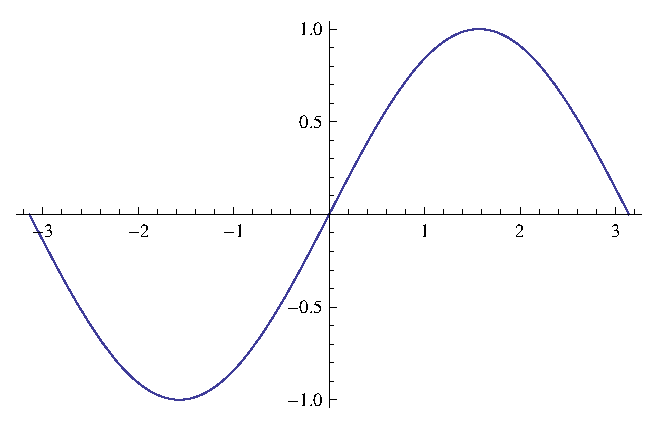
\includegraphics[scale=#1]{temp12_figs/sample.eps}
\mfigbicap{#3}{#4}\label{#5} 
\end{figure}
}}

\newcommand{\mfigTwo}[7]{                      
\ifthenelse{\boolean{flag_plot}}{\begin{figure}[H]
\centering                                    
\includegraphics[scale=#1]{#2}
\includegraphics[scale=#3]{#4}
\mfigbicap{#5}{#6}\label{#7}
\end{figure}}{\begin{figure}[H]
\centering 
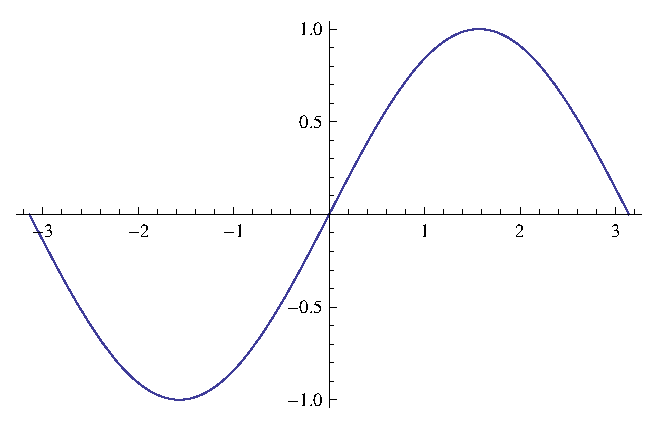
\includegraphics[scale=#1]{temp12_figs/sample.eps}
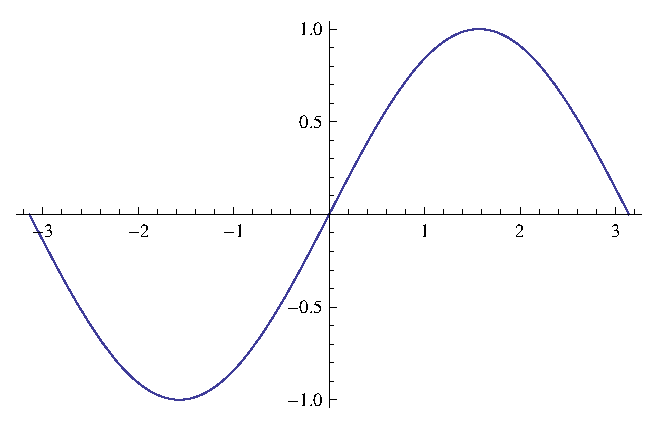
\includegraphics[scale=#3]{temp12_figs/sample.eps}
\mfigbicap{#5}{#6}\label{#7} 
\end{figure}
}}


\newcommand{\mfigThr}[9]{                      
\ifthenelse{\boolean{flag_plot}}{\begin{figure}[H]
\centering                                    
\includegraphics[scale=#1]{#2}
\includegraphics[scale=#3]{#4}
\includegraphics[scale=#5]{#6}
\mfigbicap{#7}{#8}\label{#9}
\end{figure}}{\begin{figure}[H]
\centering 
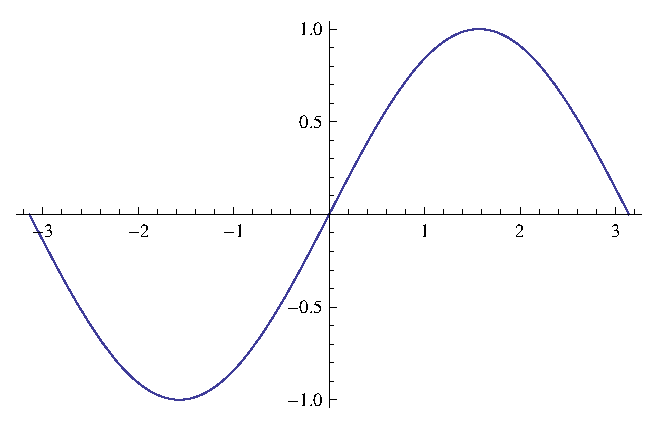
\includegraphics[scale=#1]{temp12_figs/sample.eps}
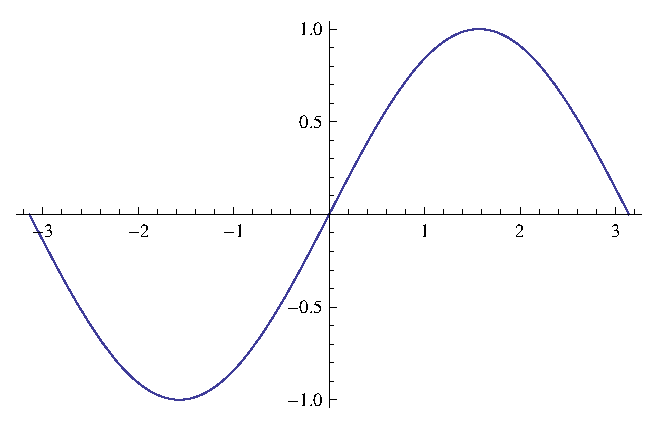
\includegraphics[scale=#3]{temp12_figs/sample.eps}
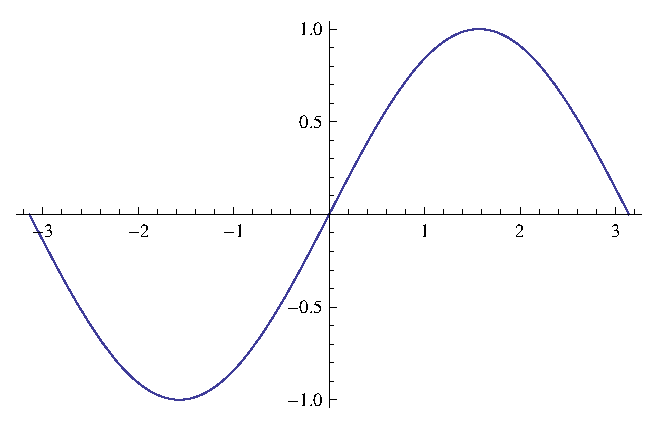
\includegraphics[scale=#5]{temp12_figs/sample.eps}
\mfigbicap{#7}{#8}\label{#9} 
\end{figure}
}}

 
\newcommand{\mfigFouLin}[8]{                      
\ifthenelse{\boolean{flag_plot}}{\begin{figure}[H]
\centering                                    
\includegraphics[scale=#1]{#2}
\includegraphics[scale=#1]{#3}
\includegraphics[scale=#1]{#4}
\includegraphics[scale=#1]{#5}
\mfigbicap{#6}{#7}\label{#8}
\end{figure}}{\begin{figure}[H]
\centering 
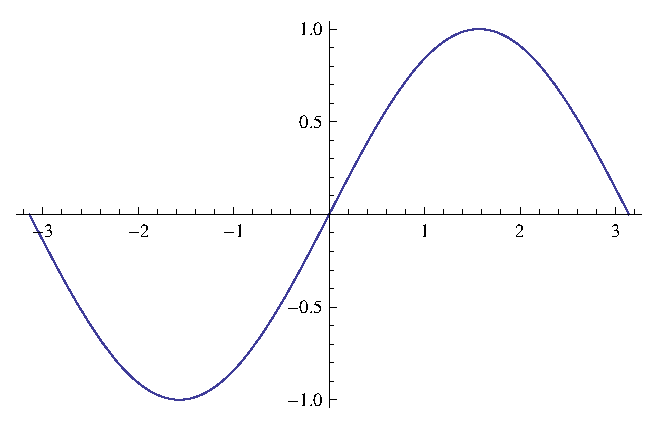
\includegraphics[scale=#1]{temp12_figs/sample.eps}
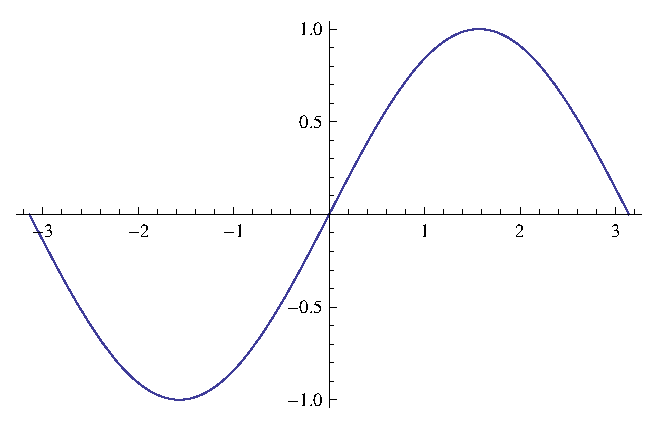
\includegraphics[scale=#1]{temp12_figs/sample.eps}
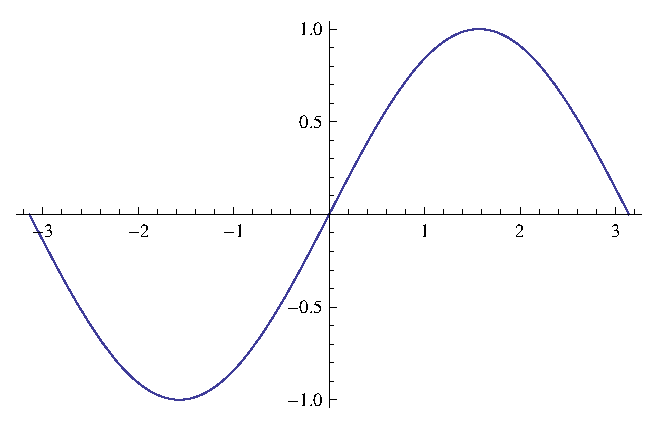
\includegraphics[scale=#1]{temp12_figs/sample.eps}
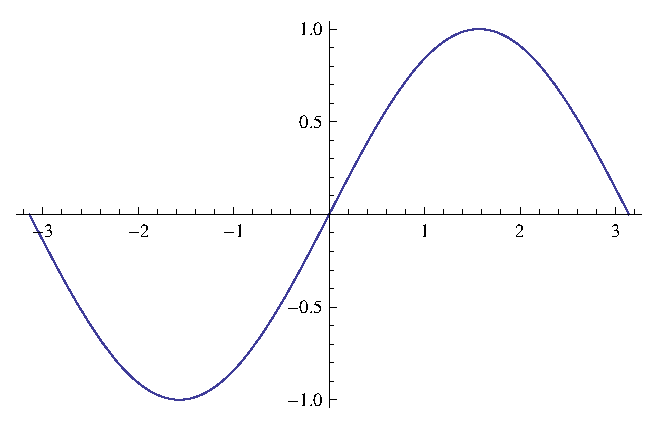
\includegraphics[scale=#1]{temp12_figs/sample.eps}
\mfigbicap{#6}{#7}\label{#8} 
\end{figure}
}}


\newcommand{\mfigFouMat}[8]{                      
\ifthenelse{\boolean{flag_plot}}{\begin{figure}[H]
\centering                                    
\includegraphics[scale=#1]{#2}
\includegraphics[scale=#1]{#3}\\
\includegraphics[scale=#1]{#4}
\includegraphics[scale=#1]{#5}
\mfigbicap{#6}{#7}\label{#8}
\end{figure}}{\begin{figure}[H]
\centering 
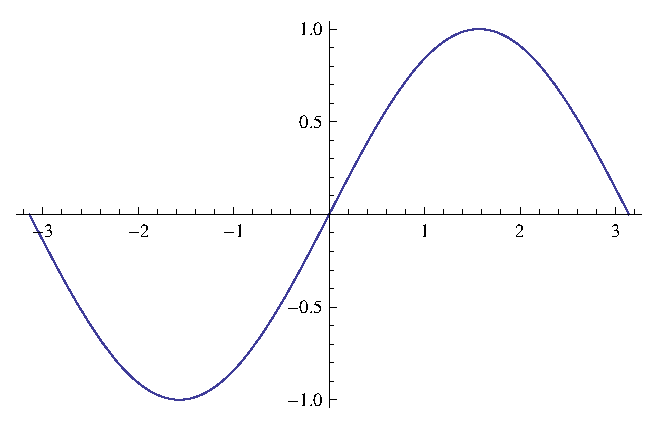
\includegraphics[scale=#1]{temp12_figs/sample.eps}
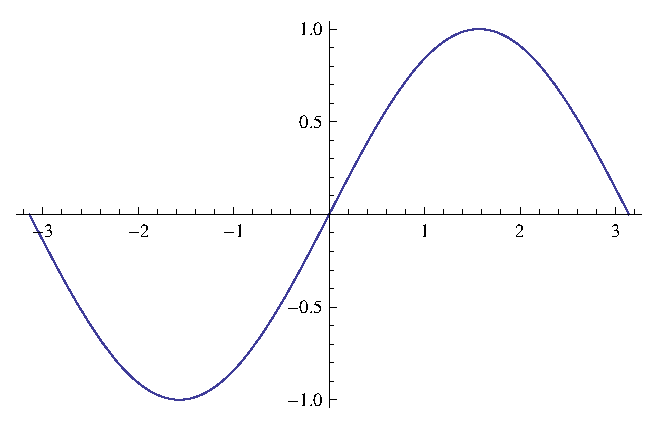
\includegraphics[scale=#1]{temp12_figs/sample.eps}\\
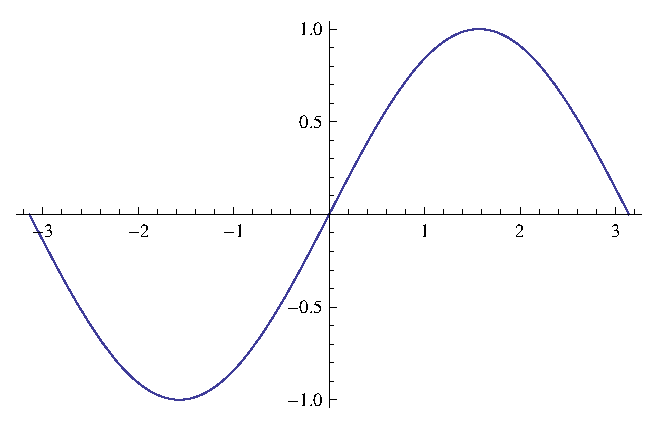
\includegraphics[scale=#1]{temp12_figs/sample.eps}
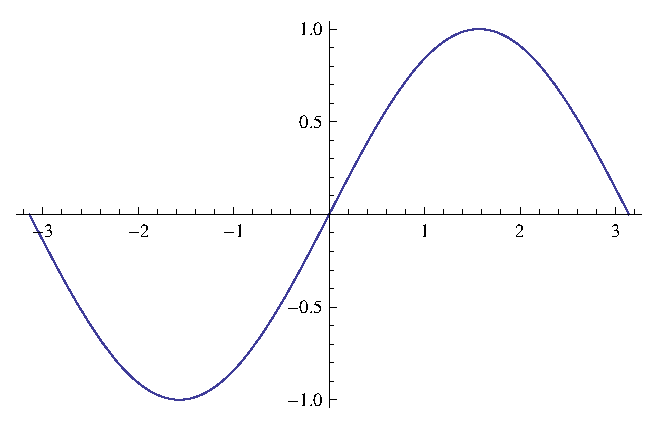
\includegraphics[scale=#1]{temp12_figs/sample.eps}
\mfigbicap{#6}{#7}\label{#8} 
\end{figure}
}}


\newcommand{\mfigFivLin}[8]{                      
\ifthenelse{\boolean{flag_plot}}{\begin{figure}[H]
\centering                                    
\includegraphics[scale=\figsizetin]{#1}
\includegraphics[scale=\figsizetin]{#2}
\includegraphics[scale=\figsizetin]{#3}
\includegraphics[scale=\figsizetin]{#4}
\includegraphics[scale=\figsizetin]{#5}
\mfigbicap{#6}{#7}\label{#8}
\end{figure}}{\begin{figure}[H]
\centering 
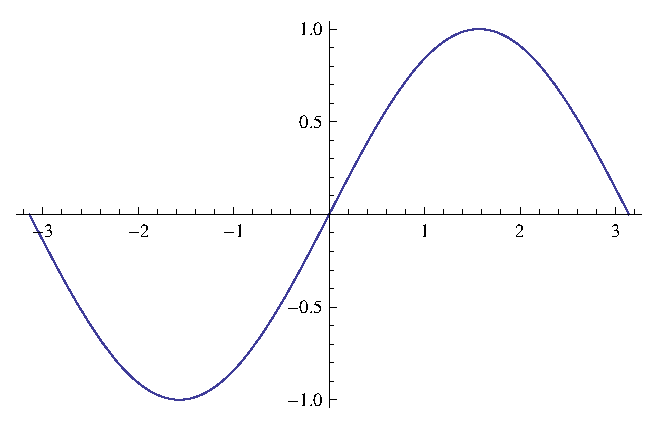
\includegraphics[scale=\figsizesma]{temp12_figs/sample.eps}
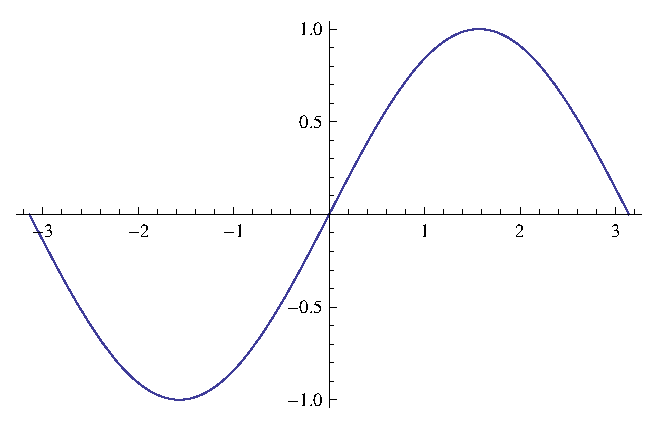
\includegraphics[scale=\figsizesma]{temp12_figs/sample.eps}
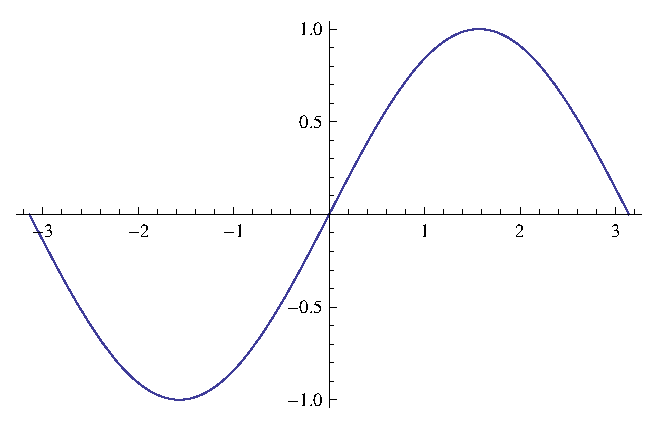
\includegraphics[scale=\figsizesma]{temp12_figs/sample.eps}
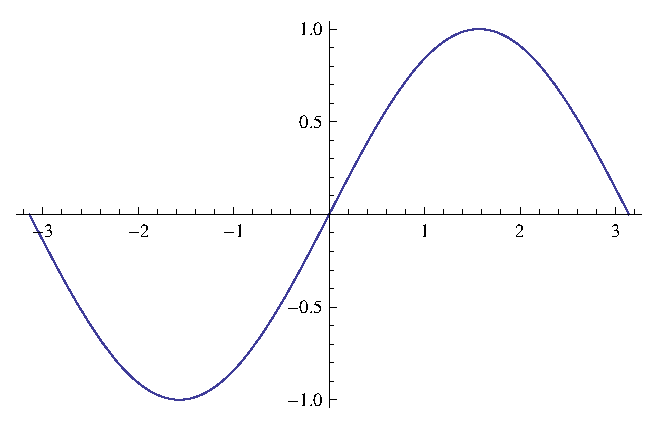
\includegraphics[scale=\figsizesma]{temp12_figs/sample.eps}
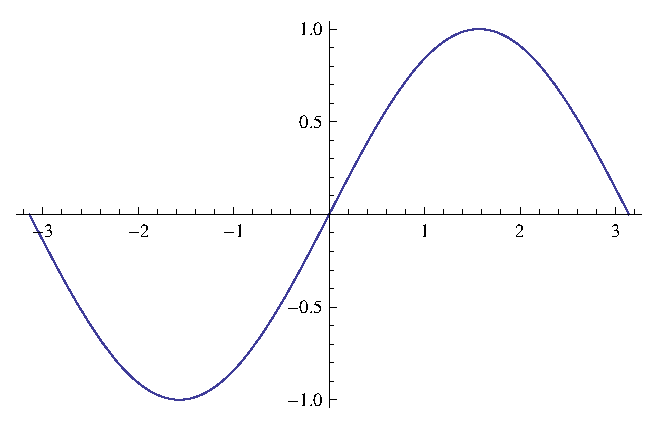
\includegraphics[scale=\figsizesma]{temp12_figs/sample.eps}
\mfigbicap{#6}{#7}\label{#8} 
\end{figure}
}}

\newcommand{\mfigSixPor}[9]{                      
\ifthenelse{\boolean{flag_plot}}{\begin{figure}[H]
\centering                                    
\includegraphics[scale=\figsizesma]{#1}
\includegraphics[scale=\figsizesma]{#2}\\
\includegraphics[scale=\figsizesma]{#3}
\includegraphics[scale=\figsizesma]{#4}\\
\includegraphics[scale=\figsizesma]{#5}
\includegraphics[scale=\figsizesma]{#6}
\mfigbicap{#7}{#8}\label{#9}
\end{figure}}{\begin{figure}[H]
\centering 
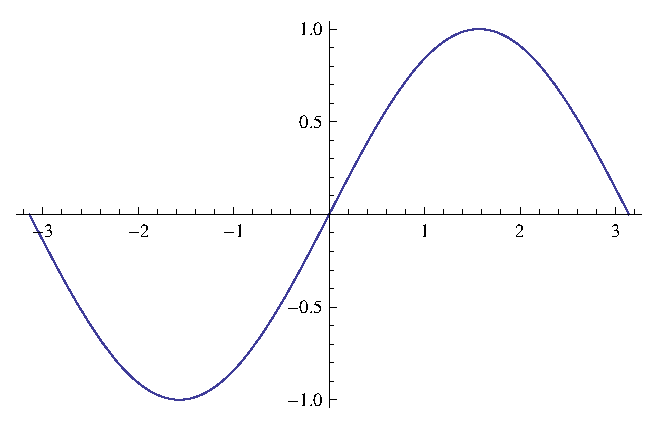
\includegraphics[scale=0.25]{temp12_figs/sample.eps}
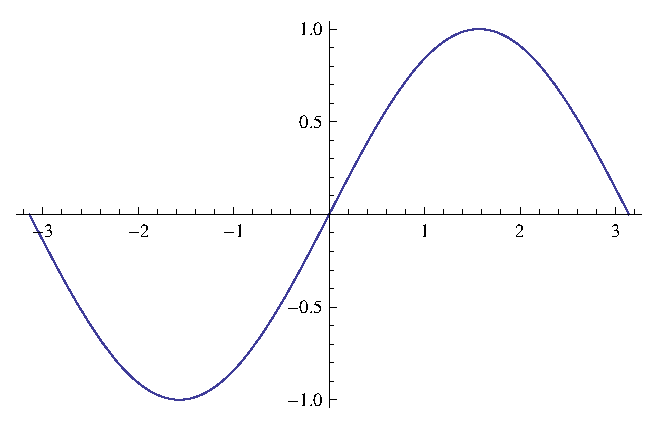
\includegraphics[scale=0.25]{temp12_figs/sample.eps}\\
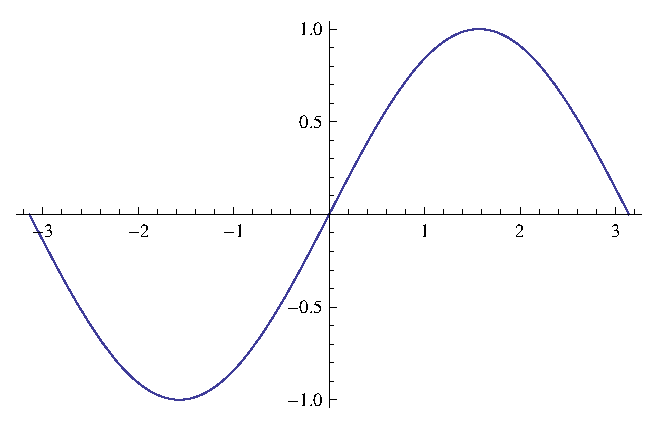
\includegraphics[scale=0.25]{temp12_figs/sample.eps}
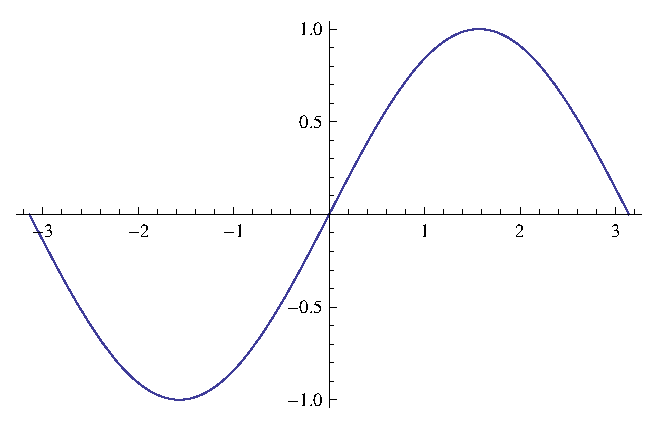
\includegraphics[scale=0.25]{temp12_figs/sample.eps}\\
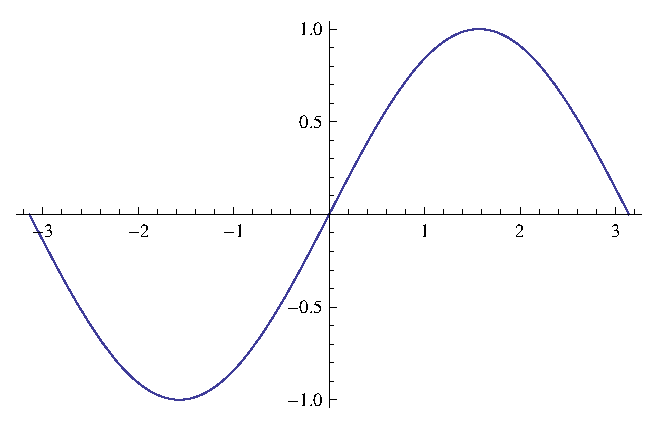
\includegraphics[scale=0.25]{temp12_figs/sample.eps}
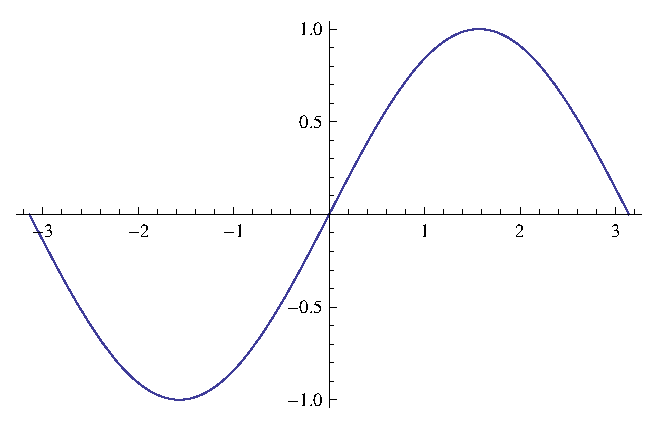
\includegraphics[scale=0.25]{temp12_figs/sample.eps}
\mfigbicap{#7}{#8}\label{#9}
\end{figure}
}}

\newcommand{\mfigSixLan}[9]{                      
\ifthenelse{\boolean{flag_plot}}{\begin{figure}[H]
\centering                                    
\includegraphics[scale=\figsizesma]{#1}
\includegraphics[scale=\figsizesma]{#2}
\includegraphics[scale=\figsizesma]{#3}\\
\includegraphics[scale=\figsizesma]{#4}
\includegraphics[scale=\figsizesma]{#5}
\includegraphics[scale=\figsizesma]{#6}
\mfigbicap{#7}{#8}\label{#9}
\end{figure}}{\begin{figure}[H]
\centering 
\includegraphics[scale=0.25]{temp12_figs/sample.eps}
\includegraphics[scale=0.25]{temp12_figs/sample.eps}
\includegraphics[scale=0.25]{temp12_figs/sample.eps}\\
\includegraphics[scale=0.25]{temp12_figs/sample.eps}
\includegraphics[scale=0.25]{temp12_figs/sample.eps}
\includegraphics[scale=0.25]{temp12_figs/sample.eps}
\mfigbicap{#7}{#8}\label{#9}
\end{figure}
}}


\makeatletter
\@addtoreset {table}{chapter}
\makeatother

\newcommand{\mtabbicap}[2]{                %жšÒåÃüÁîfigbicap ÉùÃ÷ÓÐÁœžö²ÎÊý (Ò»žöÖÐÎıêÌâÒ»žöÓ¢ÎıêÌâ)
\renewcommand{\tablename}{表.}                %œ«figureÀàµÄÃû×ÖžÄΪÖÐÎĵÄ"ÍŒ"
\caption{#1}                                  %œ«µÚÒ»žö±äÁ¿Êä³öΪ͌ƬµÄµÚÒ»±êÌâ, ÓÉÓÚÉÏÃæÉèÖÃÁË"ÍŒ" ËùÒÔµÚÒ»±äÁ¿ÊÇÖÐÎıêÌâ, ŸÍÊÇÕâ¶ùµÄ#1
\addtocounter{table}{-1}                     %œ«figureŒÆÊýÆ÷ŒõÒ», ÕâÑùÊä³öµÚ¶þÓ¢ÎıêÌâµÄʱºòÄܺÍÖÐÎıêÌâ±£³Ö±àºÅÒ»ÖÂ
\vspace{-1.8ex}                               %œ«ÁœžöcapµÄÐÐŒäŸàŒõÉÙ0.5ex
\renewcommand{\tablename}{Tab.}              %œ«figureÀàµÄÃû×ÖžÄΪӢÎĵÄ"Fig"
\caption{#2}
\vspace{-0.1ex}                                  %ͬÖÐÎĵڶþ²œ
}

\newcommand{\mtab}[4]{                      %¶šÒåÒ»žöHEUµÄ²å±íÃüÁÆäÖÐÓÐ4žöÊäÈ룬·Ö±ðÊÇÖÐÎĵıêÌ⣬ӢÎĵıêÌ⣬ÒýÓõıêÇ©ºÍ±ížñµÄÄÚÈÝ¡£
\begin{table}[H]                              %modified on : 16:49 2011-3-21.×ÔŒº¶šÒåµÄ¡£
\mtabbicap{#1}{#2}\label{#3}                %\caption{²âÊÔº¯Êý}\label{t_benchmark}
\centering                                    %ŸÓÖÐÏÔÊŸ ±ŸÀŽÓõÄÊÇ\begin{center}ºÍ\end{center}µÄ£¬µ«Ö®ºóµÄ¿Õ°×Ì«Žó£¬ŸÍžÄÓÃÕâžöÁË¡£
\begin{tiny}
\input{#4}
\end{tiny}
\end{table}
}


